\section{Bar plot of Types} \label{appendix:types-barplot}
The bar plot over the types is a result of the EDA performed.
It helps visualising why \texttt{StratifiedKFold} might be more reasonable to use than the standard \texttt{KFold} method, as the data set is imbalanced.

\begin{figure}[htp] 
    \centering
    \caption{Bar plot showing the number of occurences in the data set for each MBTI.}
    \label{fig:types-barplot}
    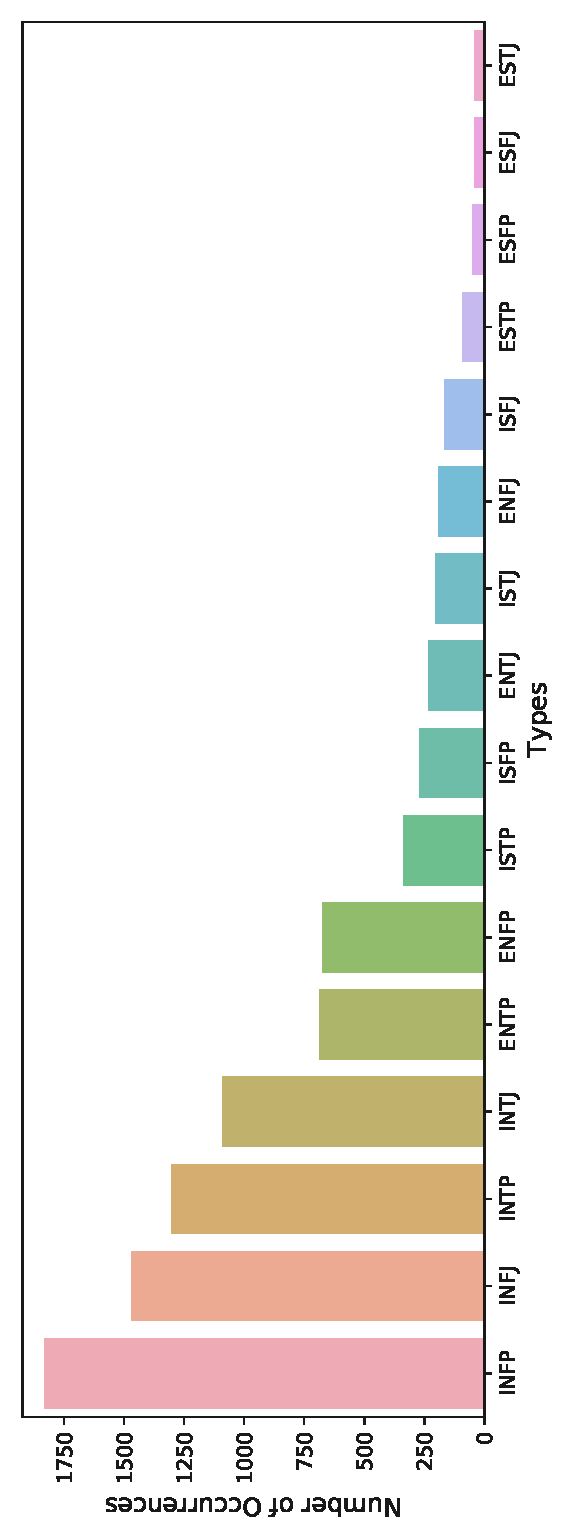
\includegraphics[scale=0.7]{types_barplot.pdf}
\end{figure}